\documentclass[a4paper]{article}

\usepackage{color}
\usepackage{url}
\usepackage[T2A]{fontenc} 
\usepackage[utf8]{inputenc}
\usepackage{graphicx}

\usepackage[english,serbian]{babel}

\begin{document}

\section{Slučaj upotrebe: Unošenje radnih sati}
\begin{enumerate}
    \item \textbf{Kratak opis:} Zaposleni unosi broj odrađenih ranih sati za konkretan dan kao i opis odrađenog posla.
    \item \textbf{Učesnici:}
        \begin{itemize}
            \item Zaposleni
        \end{itemize}
    \item \textbf{Preduslovi:} Zaposleni je registrovani korisnik sistema i nije unet odrađen broj radnih sati za dan koji korisnik popunjava.
    \item \textbf{Postuslovi:} Odrađen broj radnih sati za konkretan dan je sačuvan u sistemu. Baza je ažurirana. Na stranici se prikazuje novi tiket koji je u nerazrešenom statusu.
    \item \textbf{Osnovni tok:}
        \begin{enumerate}
            \item Zaposleni otvara stranicu gde se prikazuju dani i uneti radni sati za te dane.
            \item Pritiska dugme za dodavanje novog dana i broja unetih radnih sati.
            \item Prikazuje se formular koji sadrži polja za odabir dana, broj odrađenih radnih sati, i opis odrađenog posla.
            \item Zaposleni popunjava formular.
            \item Potvrđuje unos za taj dan.
            \item Sistem vrši obradu podataka.
            \item Sistem čuva unete podatke u bazi podataka.
            \item Na stranici se dodaje tiket koji je u nerazrešenom statusu i informacije koje je korisnik uneo za taj dan.
        \end{enumerate}
    \item \textbf{Alternativni tokovi:}
        \begin{enumerate}
            \item \textbf{Zaposleni je odabrao nevalidan dan}. Ukoliko u koraku (d) korisnik odabere dan za koji je uneo radne sate ili dan koji je ispred trenutnog dana, prikazuje mu se odgovarajuća poruka o grešci. Proces se nastavlja u koraku (d).
            \item \textbf{Zaposleni je odabrao nevalidan broj radnih sati}. Ukoliko u koraku (d) zaposleni unese radne sate koji predstavljaju negativan broj, prikazuje mu se odgovarajuća poruka o grešci. Proces se nastavlja u koraku (d).
        \end{enumerate}
    \item \textbf{Podtokovi:} /
    \item \textbf{Specijalni zahtevi:} /
    \item \textbf{Dodatne informacije:} Polje za unosenje broja radnih sati je obavezno.
\end{enumerate}


\includegraphics[scale=0.5]{PrijavljivanjeRadnogVremena.jpg}

\section{Slučaj upotrebe: Izmena tiketa}
\begin{enumerate}
    \item \textbf{Kratak opis:} Zaposleni menja informacije u tiketu za konkretan dan.
    \item \textbf{Učesnici:}
        \begin{itemize}
            \item Zaposleni
        \end{itemize}
    \item \textbf{Preduslovi:} Tiket za dan čije informacije korisnik menja je prikazan na stranici, postoji u sistemu i u nerazrešenom je statusu.
    \item \textbf{Postuslovi:} Informacije su ažurirane u sistemu i korisnik vidi promene na tiketu za dan koji je ažurirao.
    \item \textbf{Osnovni tok:}
        \begin{enumerate}
            \item Zaposleni otvara stranicu gde se prikazuju dani i uneti radni sati za te dane.
            \item Pritiska odgovarajuće dugme za izmenu podataka na tiketu.
            \item Na tiketu polja za unošenje radnih sati i opis odrađenog posla postaju moguća za izmenu.
            \item Zaposleni menja odgovarajuća polja.
            \item Potvrđuje izmene.
            \item Sistem vrši obradu podataka.
            \item Sistem čuva unete podatke u bazi podataka.
            \item Na stranici se prikazuje tiket u izmenjenom obliku.
        \end{enumerate}
    \item \textbf{Alternativni tokovi:}
        \begin{enumerate}
            \item \textbf{Zaposleni je odabrao nevalidan broj radnih sati}. Ukoliko u koraku (d) zaposleni unese radne sate koji predstavljaju negativan broj, prikazuje mu se odgovarajuća poruka o grešci. Proces se nastavlja u koraku (d).
        \end{enumerate}
    \item \textbf{Podtokovi:} /
    \item \textbf{Specijalni zahtevi:} /
    \item \textbf{Dodatne informacije:} Polje za unosenje broja radnih sati je obavezno.
\end{enumerate}
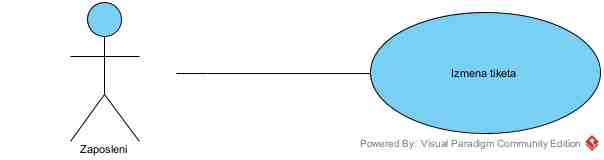
\includegraphics[scale=0.5]{IzmenaTiketa.jpg}

\end{document}
